\documentclass[tikz,border=8pt]{standalone}
% Shared look for every TikZ diagram. Load with \input{../../tools/tikz-style.tex}
\usepackage[T1]{fontenc}
\usepackage{lmodern}
\renewcommand{\sfdefault}{lmr}  % diagrams use the same serif as the text
\usetikzlibrary{arrows.meta, positioning, shapes.geometric, calc, fit, backgrounds}
\definecolor{cblue}{HTML}{4C78A8}
\definecolor{corange}{HTML}{F58518}
\definecolor{cgreen}{HTML}{54A24B}
\definecolor{cred}{HTML}{E45756}
\definecolor{cpurple}{HTML}{B279A2}
\definecolor{cgrey}{HTML}{6B6B6B}
\tikzset{
  every picture/.style={font=\sffamily, line width=1.2pt},
  box/.style={draw=#1, fill=#1!12, rounded corners=4pt, align=center, inner sep=7pt, minimum height=1.1cm},
  box/.default=cgrey,
  arrow/.style={-{Stealth[length=3mm]}, draw=cgrey, line width=1.4pt},
  title/.style={font=\sffamily\bfseries\Large},
  note/.style={font=\sffamily\small, text=cgrey, align=center},
}
\AtBeginDocument{\hyphenpenalty=10000 \exhyphenpenalty=10000}

\begin{document}
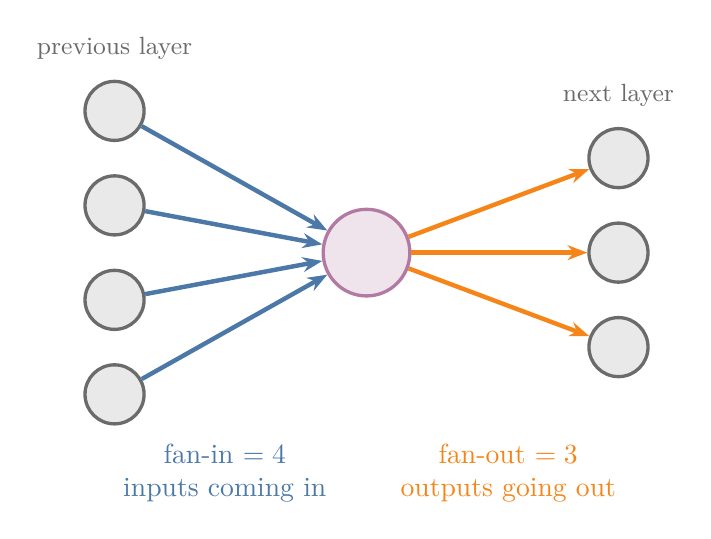
\begin{tikzpicture}[
  n/.style={circle, draw=cgrey, fill=cgrey!15, minimum size=0.75cm, inner sep=0pt},
  me/.style={circle, draw=cpurple, fill=cpurple!20, minimum size=1.1cm, inner sep=0pt}]
  \foreach \i/\yy in {1/1.8, 2/0.6, 3/-0.6, 4/-1.8} \node[n] (a\i) at (0,\yy) {};
  \node[me] (m) at (3.2,0) {};
  \foreach \j/\yy in {1/1.2, 2/0, 3/-1.2} \node[n] (b\j) at (6.4,\yy) {};
  \foreach \i in {1,...,4} \draw[cblue, line width=1.6pt, -{Stealth[length=2.5mm]}] (a\i) -- (m);
  \foreach \j in {1,2,3} \draw[corange, line width=1.6pt, -{Stealth[length=2.5mm]}] (m) -- (b\j);
  \node[font=\sffamily, text=cblue, align=center] at (1.4,-2.8) {fan-in $= 4$\\inputs coming in};
  \node[font=\sffamily, text=corange, align=center] at (5.0,-2.8) {fan-out $= 3$\\outputs going out};
  \node[font=\sffamily\small, text=cgrey] at (0,2.6) {previous layer};
  \node[font=\sffamily\small, text=cgrey] at (6.4,2.0) {next layer};
\end{tikzpicture}
\end{document}
